% !TEX encoding = UTF-8 Unicode
\documentclass{standalone}
% \usepackage{pgfplots}
% \pgfplotsset{compat=1.11}

\renewcommand{\familydefault}{\sfdefault}
% \usepackage[version=0.96]{pgf}
\usepackage{tikz}
% \usetikzlibrary{arrows,shapes,automata,backgrounds,petri,positioning}
% \usetikzlibrary{decorations.pathmorphing}
% \usetikzlibrary{decorations.shapes}
% \usetikzlibrary{decorations.text}
% \usetikzlibrary{decorations.fractals}
% \usetikzlibrary{decorations.footprints}
% \usetikzlibrary{shadows}
% \usetikzlibrary{calc}
% \usetikzlibrary{spy}

% \pgfplotsset{compat=1.11}
\usepackage[utf8]{inputenc}
% \usepackage[vietnam]{babel}

\def\d{.6}
% \def\p{5.1}
\def\q{-.6}
% \def\sc{25}

\newcommand{\nn}[4]{
    \begin{scope}[xshift = #1*\d cm, yshift = #2*\q cm]
        
    \node at (0, 0) [anchor = east, draw, inner sep = 0, fill = #3!20, minimum height = .6cm, minimum width = .6cm] {#4};
    \end{scope}
}

\newcommand{\nnn}[4]{
    \begin{scope}[xshift = #1*\d cm, yshift = #2*\q cm]
        
    \node at (0, 0) [anchor = east, align = left,  draw, inner sep = 0, fill = #3!30, minimum height = .6cm, minimum width = .6cm] {#4};
    \end{scope}
}



\begin{document}
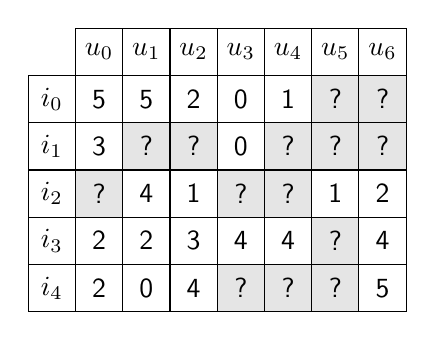
\begin{tikzpicture}
    \nn{1}{0}{white}{${u}_0$};
    \nn{1}{1}{white}{5};
    \nn{1}{2}{white}{3};
    \nn{1}{3}{gray}{?};
    \nn{1}{4}{white}{2};
    \nn{1}{5}{white}{2};

    \nn{2}{0}{white}{${u}_1$};
    \nn{2}{1}{white}{5};
    \nn{2}{2}{gray}{?};
    \nn{2}{3}{white}{4};
    \nn{2}{4}{white}{2};
    \nn{2}{5}{white}{0};

    \nn{3}{0}{white}{${u}_2$};
    \nn{3}{1}{white}{2};
    \nn{3}{2}{gray}{?};
    \nn{3}{3}{white}{1};
    \nn{3}{4}{white}{3};
    \nn{3}{5}{white}{4};

    \nn{4}{0}{white}{${u}_3$};
    \nn{4}{1}{white}{0};
    \nn{4}{2}{white}{0};
    \nn{4}{3}{gray}{?};
    \nn{4}{4}{white}{4};
    \nn{4}{5}{gray}{?};

    \nn{5}{0}{white}{${u}_4$};
    \nn{5}{1}{white}{1};
    \nn{5}{2}{gray}{?};
    \nn{5}{3}{gray}{?};
    \nn{5}{4}{white}{4};
    \nn{5}{5}{gray}{?};

    \nn{6}{0}{white}{${u}_5$};
    \nn{6}{1}{gray}{?};
    \nn{6}{2}{gray}{?};
    \nn{6}{3}{white}{1};
    \nn{6}{4}{gray}{?};
    \nn{6}{5}{gray}{?};

    \nn{7}{0}{white}{${u}_6$};
    \nn{7}{1}{gray}{?};
    \nn{7}{2}{gray}{?};
    \nn{7}{3}{white}{2};
    \nn{7}{4}{white}{4};
    \nn{7}{5}{white}{5};


    \nnn{0}{1}{white}{${i}_0$};
    \nnn{0}{2}{white}{${i}_1$};
    \nnn{0}{3}{white}{${i}_2$};
    \nnn{0}{4}{white}{${i}_3$};
    \nnn{0}{5}{white}{${i}_4$};
   
\end{tikzpicture}
\end{document}